\documentclass{article}
\usepackage{amsmath, amssymb}
\usepackage{hyperref}
\usepackage{graphicx}
\usepackage{booktabs}
\usepackage{geometry}
\usepackage{xcolor}
\usepackage{multirow}



\geometry{margin=1in}
\title{Review of iClusterVB: A Fast Integrative Clustering and Feature Selection Approach for High-Dimensional Data}
\author{Hadiseh Azadehyaei (T00726889) \\ Feng Gu (T00751197)}
\date{Winter 2025}

\begin{document}

\maketitle

% \section{Abstract}
% Our aim is to explore the R package introduced in the project and try to
% apply this novel framework to other related datasets. The topic of this project comes from 
% the data science seminar on February 5, 2024. The detailed information is as follows:

% \begin{itemize}
%     \item \textbf{Topic:} iClusterVB: A fast integrative clustering and feature selection approach for high-dimensional data
%     \item \textbf{Date:} 5 February 2024
%     \item \textbf{Speaker:} Dr. Zihang Lu, Department of Public Health Sciences and Department of Mathematics and Statistics, Queen's University
%     \item \textbf{Presentation:} Given on February 5, 2024, by Dr. Zihang Lu from Queen's University
% \end{itemize}

% \section{Introduction}
Clustering analysis plays a fundamental role in revealing hidden patterns in complex biological data. It involves grouping similar data points such that those within a cluster are more similar to each other than to those in other clusters. In the field of bioinformatics, clustering has proven instrumental in tasks such as disease subtyping, biomarker discovery, and patient stratification—essential steps toward personalized medicine. Notable successes include the identification of distinct subtypes in diseases such as asthma, Parkinson’s disease, and various cancers, where clustering has enabled deeper biological insights and guided downstream predictive modeling.

However, the increasing complexity and volume of biomedical data have introduced new challenges that traditional clustering methods—such as k-means or hierarchical clustering—are often not well-equipped to address. Modern datasets, particularly in genomics and cancer research, are frequently multimodal, combining data from gene expression, DNA methylation, miRNA expression, mutations, and more. These data types vary in structure—continuous, binary, categorical—and span tens of thousands of features, only a fraction of which are typically informative. This high dimensionality and heterogeneity demand advanced statistical methods capable of integrative analysis and feature selection across multiple data views.

Integrative clustering methods have emerged as a powerful solution to these challenges 
by simultaneously analyzing multiple data types to identify robust, biologically meaningful
subtypes. Among the most promising approaches are Bayesian frameworks, 
which incorporate prior knowledge to improve inference quality. 
While traditional Bayesian methods often rely on computationally intensive 
techniques such as Markov Chain Monte Carlo (MCMC), more recent developments like
 Variational Bayes (VB) provide faster and more scalable alternatives by transforming 
 the inference task into an optimization problem.

The iClusterVB R package, introduced by Alnajjar and Lu (2024), leverages a
 variational Bayesian approach to enable efficient integrative clustering and 
 feature selection in high-dimensional, mixed-type data. The package builds upon the 
 strengths of earlier tools like iClusterPlus and iClusterBayes while addressing
  their computational limitations. Key features of iClusterVB include support for continuous,
   discrete, and categorical data types; automatic selection of the optimal number of clusters;
    and a scalable algorithm well-suited for modern multi-omics applications.

In this review, we aim to assess the practical utility and generalizability of 
the iClusterVB method by applying it to both simulated data and a real-world dataset: 

\textcolor{red}{
Waiting to be added: describe the real data set or explain the simulated data set.}

% moving it to vscode for copilot refining

\section{Data source and data description}

In this section, we demonstrate the functionality of \texttt{iClusterVB} for integrative clustering and feature selection using a simulated multi-omic dataset. This simulation is designed to closely mimic the structure of real-world biological data typically encountered in genomics and precision medicine studies.

The simulated dataset includes data from \( N = 240 \) individuals, each with measurements across \( R = 4 \) different data types. Specifically, two of these data types represent \textbf{continuous variables}---such as gene or mRNA expression levels---while the third data type consists of \textbf{count data}, resembling DNA copy number variations. The fourth data type is \textbf{binary}, capturing the presence or absence of mutations or other genomic aberrations. This combination of data types reflects a common setup in integrative genomic analyses, where multiple omic layers are collected for each subject.

We assume that the underlying true structure of the data consists of \( K = 4 \) distinct clusters, corresponding to four biological subgroups. These clusters are \textbf{balanced in size}, meaning each cluster contains 25\% of the individuals (\( \pi_1 = \pi_2 = \pi_3 = \pi_4 = 0.25 \)).

Each data type contains \( p_r = 500 \) features, for a total of \( p = 2000 \) features across all data types. Among these, \textbf{only 10\%} (i.e., 50 features per data type) are informative and contribute to the clustering structure. These informative features are also referred to as \textbf{relevant or discriminative features}, as they capture the variations that distinguish between clusters. The remaining 90\% of the features in each data type serve as \textbf{irrelevant noise features}, which do not contribute to the clustering and are expected to be filtered out during the feature selection process.

The distribution of these useful features across the four clusters is structured, and the table below summarizes how the relevant features are assigned within each cluster and data type.

\begin{table}[ht]
\centering
\caption{Distribution of relevant and noise features across clusters in each data view of the simulated data}
\label{tab:simulated_data}
\begin{tabular}{|l|l|l|}
\hline
\textbf{Data View} & \textbf{Cluster} & \textbf{Distribution} \\
\hline
\multirow{5}{*}{1 (Continuous)} 
& Cluster 1 & $\mathcal{N}(10, 1)$ (Relevant) \\
& Cluster 2 & $\mathcal{N}(5, 1)$ (Relevant) \\
& Cluster 3 & $\mathcal{N}(-5, 1)$ (Relevant) \\
& Cluster 4 & $\mathcal{N}(-10, 1)$ (Relevant) \\
& -         & $\mathcal{N}(0, 1)$ (Noise) \\
\hline
\multirow{5}{*}{2 (Continuous)} 
& Cluster 1 & $\mathcal{N}(-10, 1)$ (Relevant) \\
& Cluster 2 & $\mathcal{N}(-5, 1)$ (Relevant) \\
& Cluster 3 & $\mathcal{N}(5, 1)$ (Relevant) \\
& Cluster 4 & $\mathcal{N}(10, 1)$ (Relevant) \\
& -         & $\mathcal{N}(0, 1)$ (Noise) \\
\hline
\multirow{5}{*}{3 (Binary)} 
& Cluster 1 & Bernoulli(0.05) (Relevant) \\
& Cluster 2 & Bernoulli(0.2) (Relevant) \\
& Cluster 3 & Bernoulli(0.4) (Relevant) \\
& Cluster 4 & Bernoulli(0.6) (Relevant) \\
& -         & Bernoulli(0.1) (Noise) \\
\hline
\multirow{5}{*}{4 (Count)} 
& Cluster 1 & Poisson(50) (Relevant) \\
& Cluster 2 & Poisson(35) (Relevant) \\
& Cluster 3 & Poisson(20) (Relevant) \\
& Cluster 4 & Poisson(10) (Relevant) \\
& -         & Poisson(2) (Noise) \\
\hline
\end{tabular}
\end{table}

\subsection{Exploratory Data Analysis (EDA)}

To identify and visualize the valid normal distributions from the simulated dataset, we performed the following sampling and testing operations:

\begin{itemize}
    \item \textbf{Random Sampling:} We randomly sampled 30 variables from each of the three different distributions (normal, poisson, and multinomial), resulting in a total of 90 variables for testing.
    \item \textbf{Statistical Testing:} For each sampled variable, we conducted the corresponding statistical tests:
    \begin{itemize}
        \item A normality test (e.g., Shapiro-Wilk test) for variables assumed to follow a normal distribution.
        \item A Poisson test for variables assumed to follow a Poisson distribution.
        \item A multinomial test for variables assumed to follow a multinomial distribution.
    \end{itemize}
    \item \textbf{Validation and Visualization:} Variables that passed their respective tests were visualized to determine whether they represent truly valid features or are merely low-probability events arising from noise distributions.
\end{itemize}

This process helps to filter out irrelevant noise features and retain only the informative variables that contribute to the clustering structure.


\begin{figure}[!h]
    \centering
    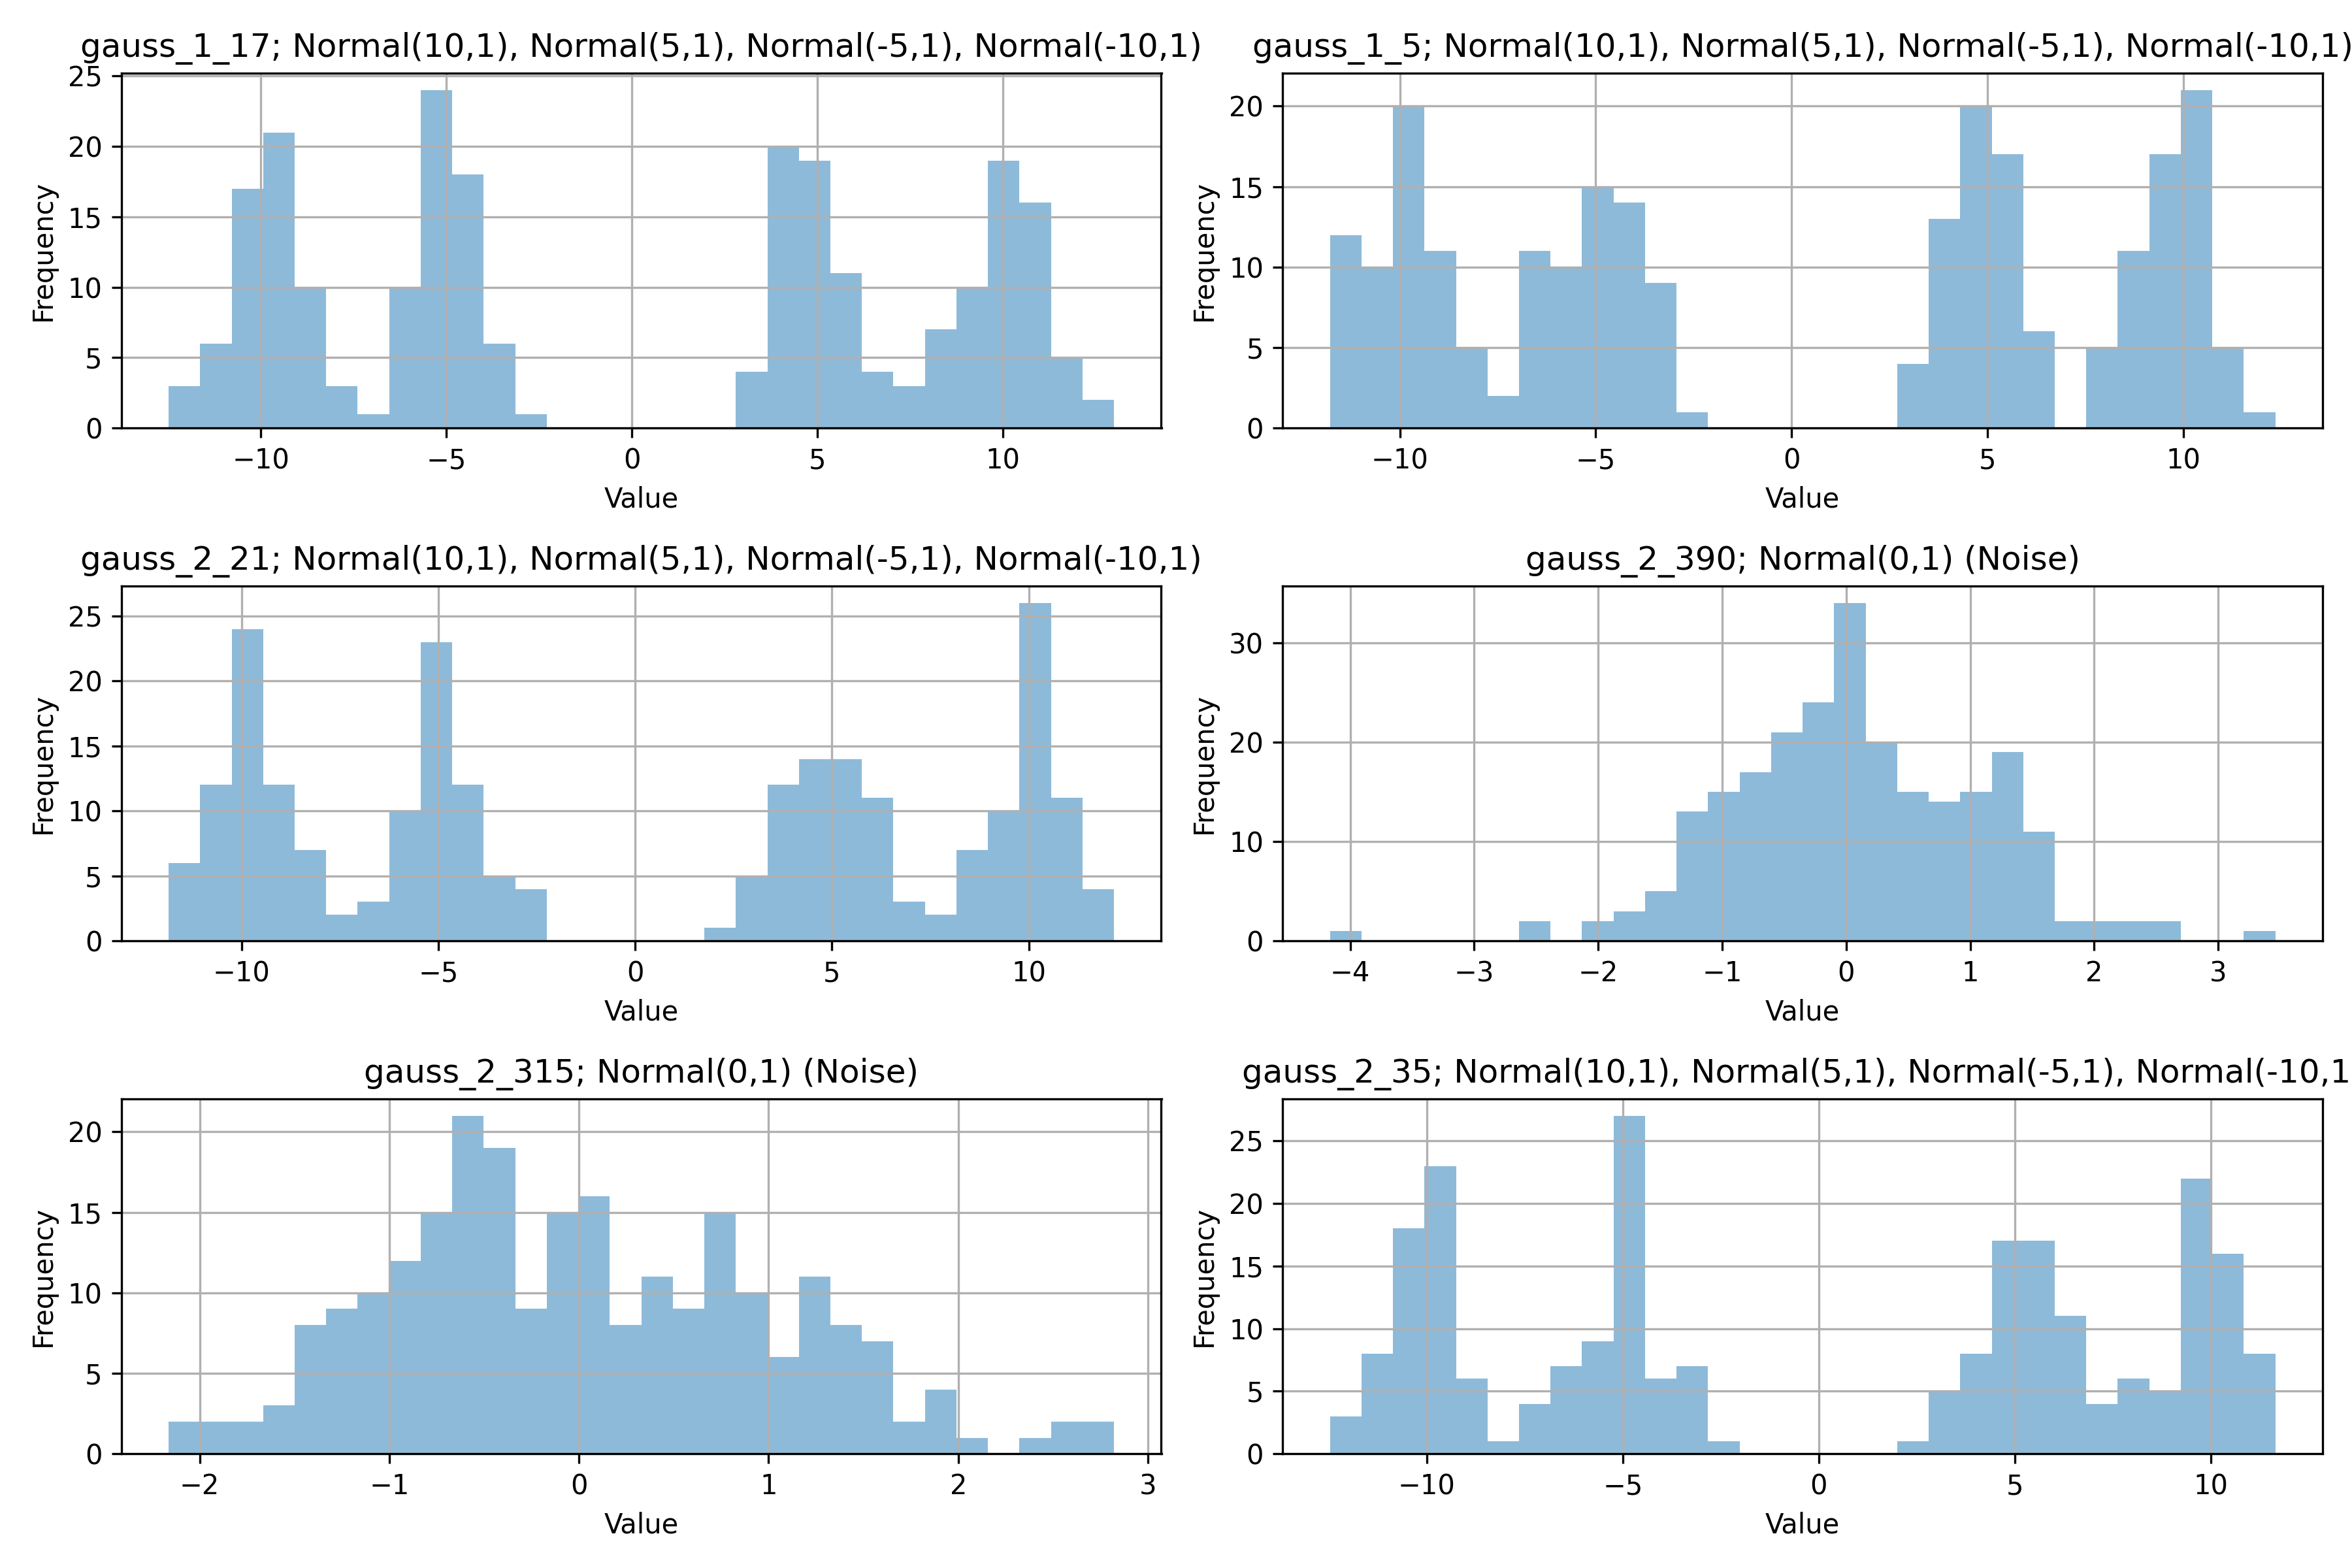
\includegraphics[width=0.9\linewidth]{../results/sim_valid_normal_distributions.png}
    \caption{Histograms of normal distributions that pass the normality test(correspond to table \ref{tab:normal_metrics})}
    \label{fig:normal_histograms}
\end{figure}

Figure~\ref{fig:normal_histograms} displays histograms of variables simulated from normal distributions.
Variables with titles including "(Noise)" correspond to noise components sampled from $\mathcal{N}(0,1)$,
while those without such a label represent relevant features derived from mixtures of $\mathcal{N}(10,1)$, 
$\mathcal{N}(5,1)$, $\mathcal{N}(-5,1)$, and $\mathcal{N}(-10,1)$. 
These relevant variables show clear multimodal patterns, indicating the presence of structured information.
In contrast, the noise variables exhibit unimodal, symmetric distributions centered around zero, 
lacking informative structure. The absence of "(Noise)" in the title marks the variables that
passed the normality test and were deemed statistically significant for downstream modeling.

\begin{figure}[!h]
    \centering
    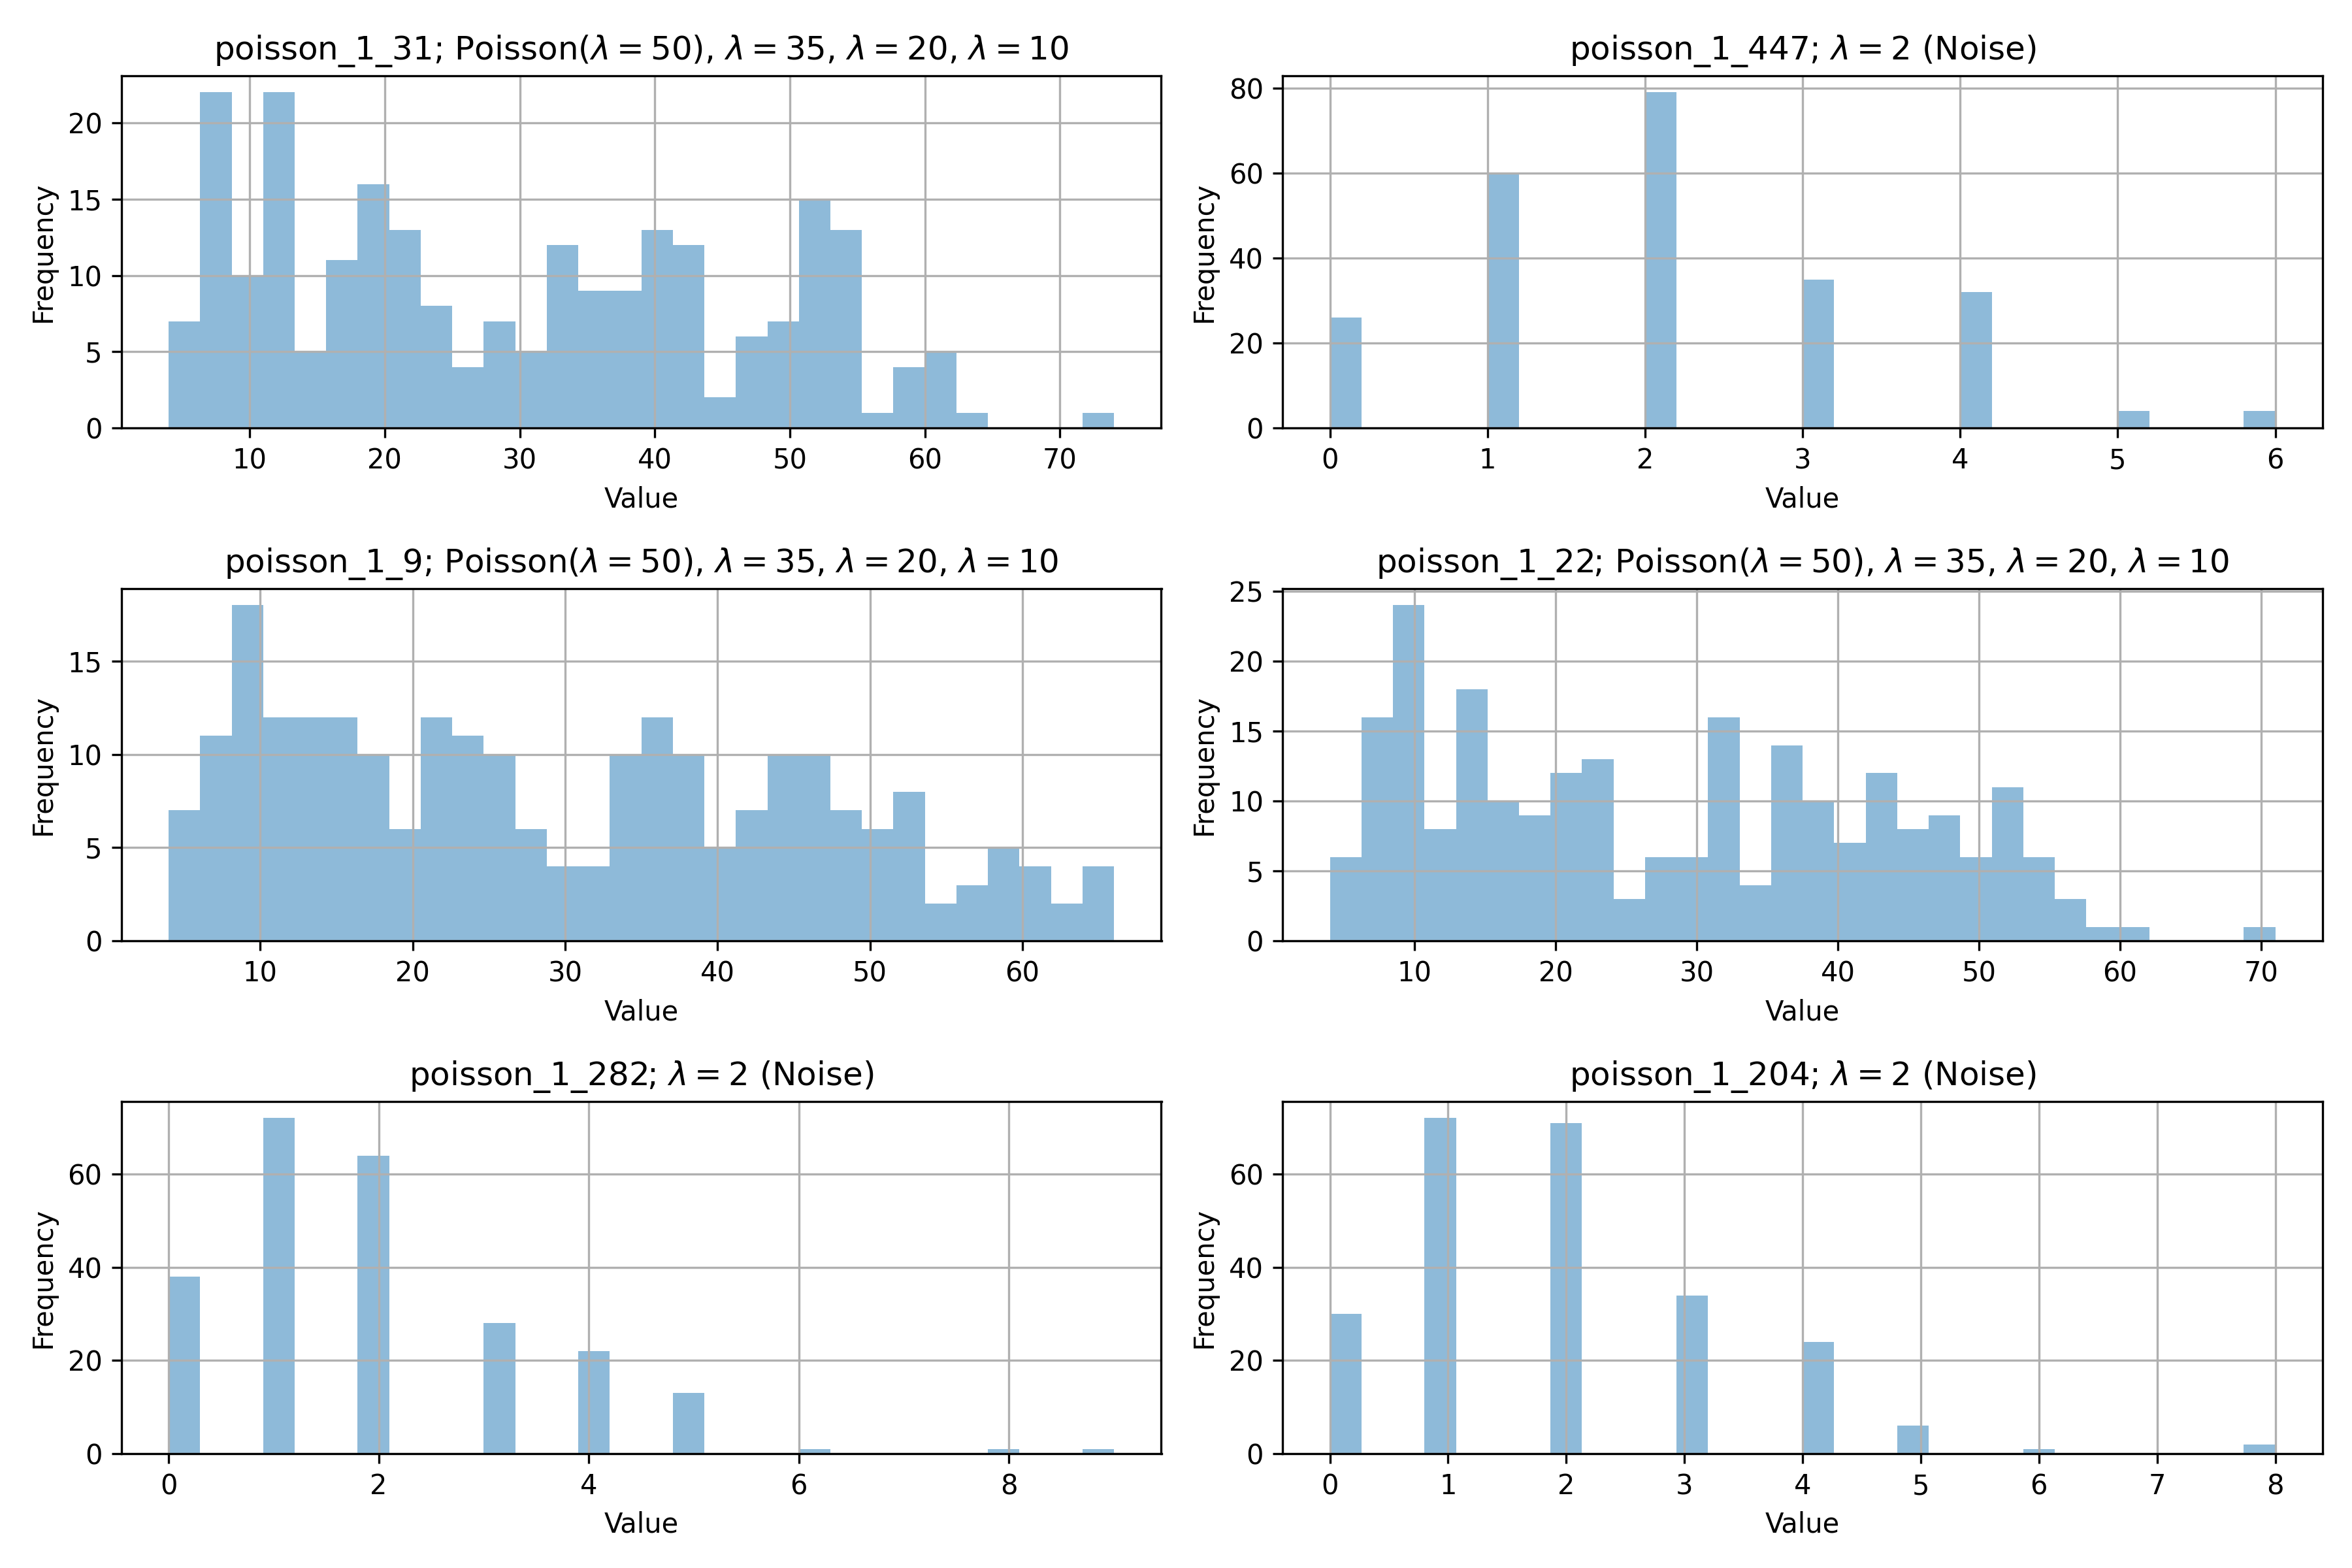
\includegraphics[width=0.9\linewidth]{../results/sim_valid_poisson_distribution.png}
    \caption{Histograms of normal distributions that pass the poission test (corresponding to table \ref{tab:poisson_metrics})}
    \label{fig:poisson_histograms}
\end{figure}

Figure~\ref{fig:poisson_histograms} shows histograms of variables generated from Poisson distributions with different
rate parameters $\lambda$. Variables labeled with multiple $\lambda$ values (e.g., $\lambda = 50, 35, 20, 10$) 
represent informative features composed of mixed Poisson signals. These histograms exhibit broader, multi-modal 
or skewed distributions, suggesting meaningful variability across groups, which is useful for clustering tasks. 
In contrast, variables marked as "(Noise)"—such as those with $\lambda = 2$ only—display narrow, 
concentrated distributions around small integer values. These noise variables do not carry discriminative 
structure and are thus considered irrelevant for clustering.

\subsection{Necessity of testing in EDA for iClusterVB algorithm}

The testing operations described above (numerical information are stored in tables \ref{tab:normal_metrics}, \ref{tab:poisson_metrics}, \ref{tab:bernoulli_metrics} in appendix) demonstrate the effectiveness of statistical tests 
in identifying suitable variables for downstream analysis. By applying normality, Poisson, and multinomial tests,
we were able to filter out irrelevant noise features and retain only the informative variables that 
exhibit meaningful patterns or variability. These selected variables are well-suited for integrative clustering 
and feature selection tasks, making them ideal candidates for input into the \texttt{iClusterVB} algorithm. 
This ensures that the algorithm operates on high-quality data, enhancing its ability to uncover biologically
meaningful clusters and informative features.



% Exploratory Data Analysis (EDA) is an important first step when working with data, especially high-dimensional data such as biological or medical datasets. EDA helps us to understand the structure of the data and to prepare it for further analysis like clustering and feature selection.

% We used EDA to look at how the data is distributed, find missing values or outliers, and see how variables relate to each other. This is useful before we apply clustering algorithms or choose important features. The methods we used here is basic  histograms or kde for each cluster. 

% \textcolor{red}{Starting here, using resampling method to check the distribution of the simulated data}


% \clearpage
% \subsection{Breast Cancer (TCGA) dataset}
% The breast cancer dataset used in this analysis was obtained from The Cancer Genome Atlas (TCGA) portal, specifically the TCGA-BRCA project, which provides comprehensive genomic data for breast cancer research. The dataset can be accessed at \url{https://portal.gdc.cancer.gov/projects/TCGA-BRCA}. This dataset includes multi-omic data, including gene expression, DNA methylation, and miRNA expression for 348 individuals diagnosed with breast cancer. The analysis was conducted using the \texttt{iClusterVB} framework, which leverages variational Bayesian inference for integrative clustering. The R code used in the analysis involved loading the necessary multi-omic data sets, specifying the clustering parameters (such as the number of clusters and feature selection method), and fitting the model using the \texttt{iClusterBayes} function. The model's posterior distributions were approximated using variational inference, and the results were visualized through heatmaps and posterior inclusion probability plots to identify informative features and cluster memberships. The \texttt{iClusterVB} framework effectively captured the heterogeneity within the dataset, revealing biologically meaningful subtypes of breast cancer based on molecular data.


% \section{iClusterVB methodology and practical steps}

\subsection{iClusterVB methodology}

The \texttt{iClusterVB} framework is built on a Bayesian model-based clustering approach using a finite mixture model, variational inference, and embedded feature selection.

\subsection{Finite Mixture Model}

A finite mixture model is a probabilistic model that represents a population as a mixture of 
several subpopulations, each described by its own probability distribution. 
It is widely used in clustering and density estimation. 
\footnote{For more details, refer 
to the \href{https://en.wikipedia.org/wiki/Mixture_model}{Wikipedia article on finite mixture models}.}

Let $\mathbf{x}_i = (x_{i1}, \ldots, x_{ip})^\top$ be the $p$-dimensional 

feature vector for individual $i$, and let $z_i$ be the cluster assignment. 
The likelihood of the data is modeled using a finite mixture model:
\[
P(\mathbf{x}_i \mid \boldsymbol{\pi}, \Theta) = \sum_{k=1}^{K} \pi_k P(\mathbf{x}_i \mid \phi_k)
\]

Assuming conditional independence of features within each cluster:

\[
P(\mathbf{x}_i \mid \phi_k) = \prod_{j=1}^{p} P(x_{ij} \mid \phi_{kj})
\]

where $\phi_k$ are parameters for the $k$-th cluster, and $\pi_k$ are mixing proportions such that $\sum_k \pi_k = 1$.

\subsection{Feature Selection}

To select informative features, the model includes a latent indicator $\gamma_{ij} \in \{0,1\}$ that controls whether feature $j$ is relevant for clustering:

\[
P(x_{ij} \mid \gamma_{ij}, z_i = k) = 
\begin{cases}
P(x_{ij} \mid \theta_{kj}), & \text{if } \gamma_{ij} = 1 \\
P(x_{ij} \mid \eta_j), & \text{if } \gamma_{ij} = 0
\end{cases}
\]

The marginal likelihood becomes:

\[
P(\mathbf{x}_i \mid z_i = k) = \prod_{j=1}^{p} \left[ \omega_j P(x_{ij} \mid \theta_{kj}) + (1 - \omega_j) P(x_{ij} \mid \eta_j) \right]
\]

where $\omega_j$ is the inclusion probability of feature $j$.

\subsection{Prior Distributions}

Priors are imposed to enable Bayesian inference, leveraging the conjugate prior method for computational efficiency and analytical tractability. Conjugate priors ensure that the posterior distribution belongs to the same family as the prior, simplifying updates during inference.

\begin{table}[h!]
\centering
\begin{tabular}{|c|c|c|c|}
\hline
\textbf{Likelihood Function} & \textbf{Parameter} & \textbf{Prior Distribution} & \textbf{Posterior Distribution} \\ \hline
$P(\mathbf{x}_i \mid \boldsymbol{\pi})$ & $\boldsymbol{\pi}$ & Dirichlet$(\alpha_0)$ & Dirichlet$(\alpha_0 + \text{counts})$ \\ \hline
$P(x_{ij} \mid \mu_{kj}, \sigma^2_{kj})$ & $\mu_{kj}$ & $\mathcal{N}(\mu_0, s_0^2)$ & $\mathcal{N}(\mu_n, s_n^2)$ \\ \hline
$P(x_{ij} \mid \sigma^2_{kj})$ & $\sigma^2_{kj}$ & $\text{IG}(a_0, b_0)$ & $\text{IG}(a_n, b_n)$ \\ \hline
$P(x_{ij} \mid \boldsymbol{\theta}_{kj})$ & $\boldsymbol{\theta}_{kj}$ & Dirichlet$(\boldsymbol{\kappa}_{kj})$ & Dirichlet$(\boldsymbol{\kappa}_{kj} + \text{counts})$ \\ \hline
$P(x_{ij} \mid \lambda_{kj})$ & $\lambda_{kj}$ & Gamma$(c_0, d_0)$ & Gamma$(c_n, d_n)$ \\ \hline
\end{tabular}
\caption{Conjugate Priors and Corresponding Posterior Distributions with Likelihood Functions and Parameters}
\label{tab:conjugate_priors}
\end{table}

\begin{itemize}
  \item \textbf{Mixing weights:} $\boldsymbol{\pi} \sim \text{Dirichlet}(\alpha_0)$ ensures that the mixing proportions are non-negative and sum to 1. The posterior updates naturally with observed cluster counts.
  \item \textbf{Gaussian features:} Conjugate priors for mean ($\mathcal{N}$) and variance ($\text{IG}$) allow efficient updates based on sufficient statistics (e.g., sample mean and variance).
  \item \textbf{Categorical features:} Dirichlet priors for multinomial parameters $\boldsymbol{\theta}_{kj}$ simplify posterior updates with observed category counts.
  \item \textbf{Count features:} Gamma priors for Poisson rates $\lambda_{kj}$ provide a flexible framework for modeling count data, with posterior updates driven by observed counts.
\end{itemize}

\subsection{Variational Inference}

  To approximate the posterior distribution $P(\beta \mid \mathbf{X})$, iClusterVB uses a method called variational inference. 
  Instead of relying on computationally expensive sampling methods, it turns the problem into an optimization task.

  The goal is to find a simpler distribution $Q(\beta)$ that is as close as possible to the true posterior
  $P(\beta \mid \mathbf{X})$. This is done by minimizing a measure called KL divergence,
  which quantifies the difference between the two distributions:

  \[
  \text{KL}(Q(\beta) \parallel P(\beta \mid \mathbf{X})) = \int Q(\beta) \log \frac{Q(\beta)}{P(\beta \mid \mathbf{X})} \, d\beta
  \]

  In practice, this is equivalent to maximizing a quantity called the Evidence Lower Bound (ELBO). The ELBO is defined as:

  \[
  \text{ELBO} = \mathbb{E}_{Q(\beta)}[\log P(\mathbf{X}, \beta)] - \mathbb{E}_{Q(\beta)}[\log Q(\beta)]
  \]

  The ELBO balances two terms: how well the model explains the data and how simple the approximating distribution is.

  Additionally, iClusterVB can automatically adjust the number of clusters by checking the estimated 
  mixing proportions $\hat{\pi}_k$. If a cluster's proportion is too small (e.g., below a threshold like 0.01),
  that cluster is removed to simplify the model.

\subsection{Practical Steps of implementing iClusterVB}

\begin{description}
  \item[Step 1: Finite Mixture Model] 
  The first step is using a finite mixture model which assumes the data arises from hidden clusters. Each cluster has its own distribution, and a latent variable determines group membership.

  \item[Step 2: Feature Selection] 
  iClusterVB performs feature selection by assigning a probability to each feature, indicating its relevance. Irrelevant features are dropped, improving interpretability.

  \item[Step 3: Prior Distributions] 
  Cluster proportions are given a Dirichlet prior. Relevant features get conjugate priors (normal/inverse gamma), while irrelevant features are estimated via MLE.

  \item[Step 4: Variational Inference] 
  Variational Bayes transforms the inference problem into an optimization task, maximizing the Evidence Lower Bound (ELBO) for faster convergence compared to MCMC.

  \item[Step 5: Model Selection] 
  The number of clusters is selected based on model fit criteria, ensuring robustness and reliability.
\end{description}

\textcolor{red}{put the code here or in the appendix}

\begin{figure}[!h]
\centering
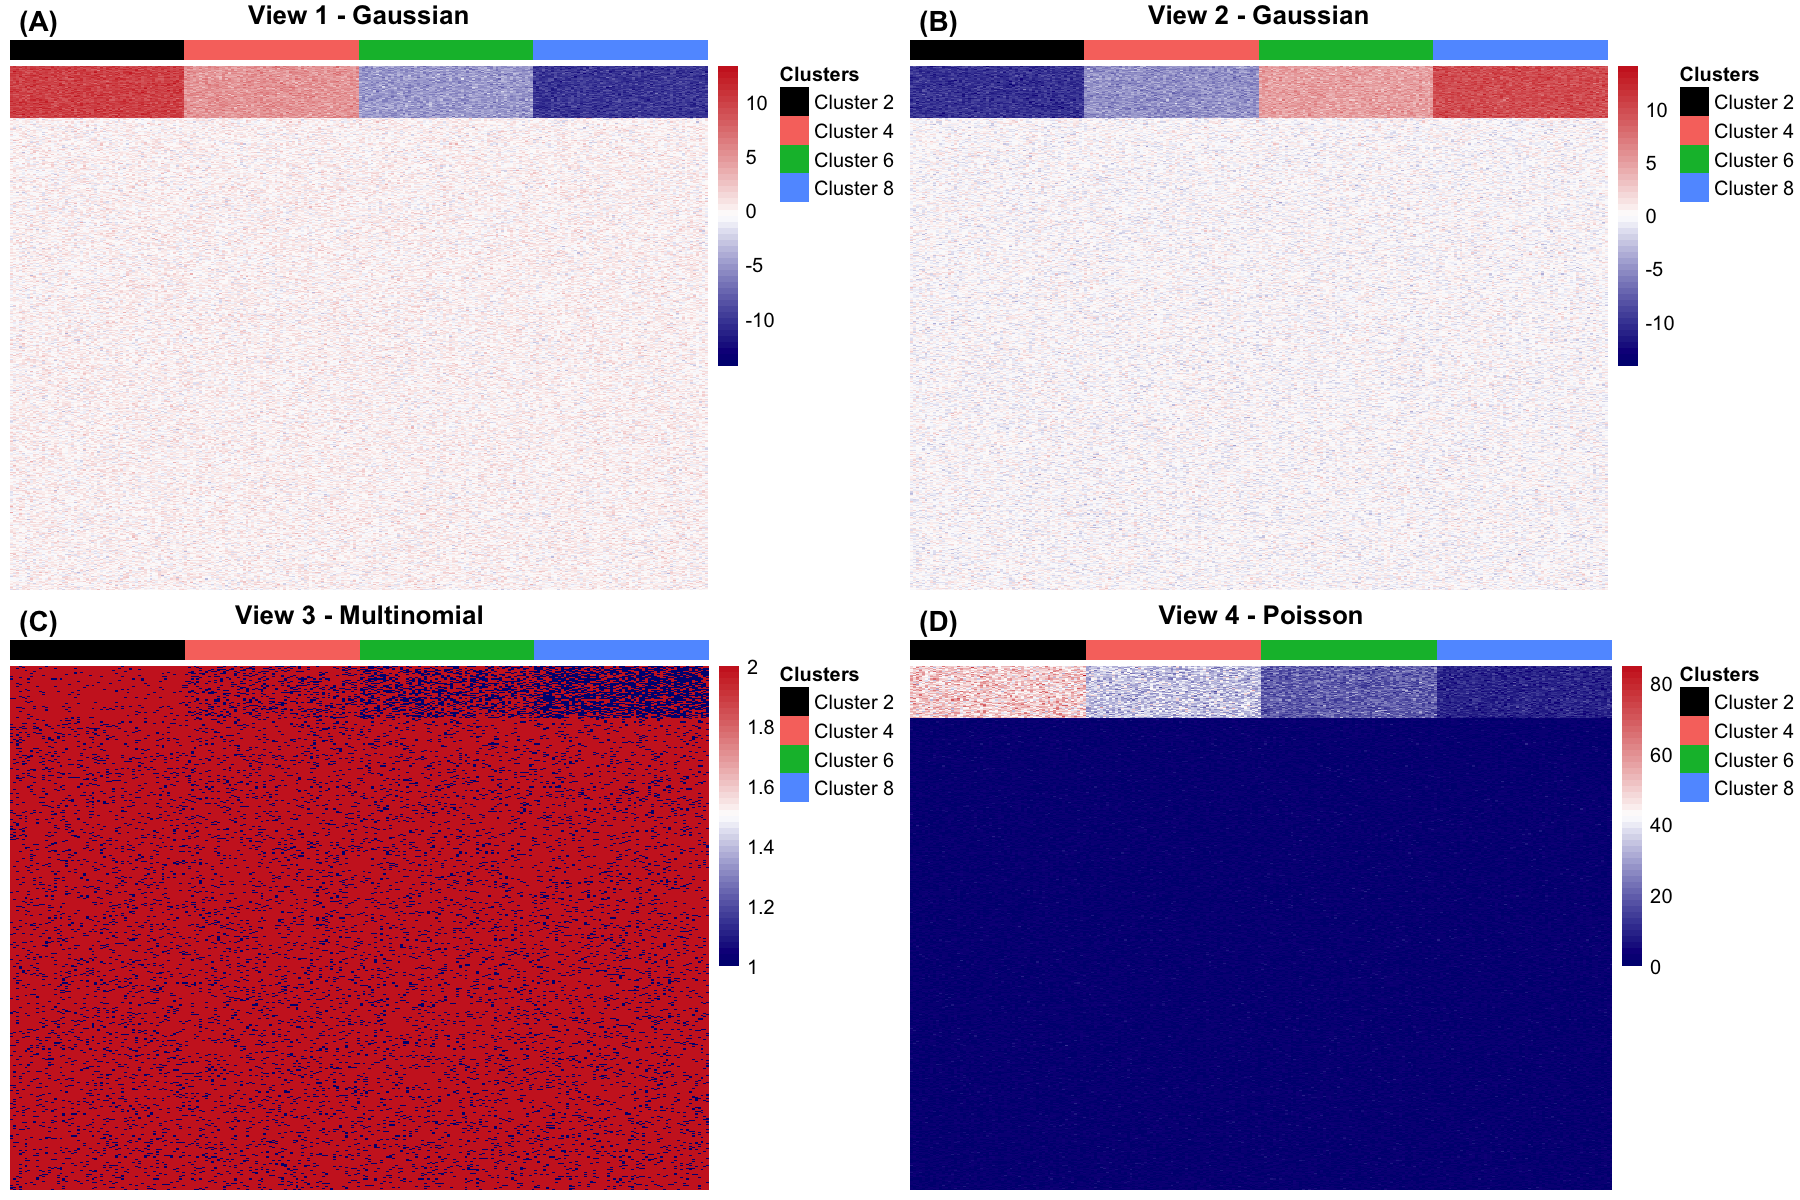
\includegraphics[width=0.9\textwidth]{../results/Simulated_heatmap.png}
\caption{Heat map of simulated data with 4 clusters}
\label{fig:simulated_heatmap}
\end{figure}
\section{iClusterVB Implementation on simulation data}

In this section, we show how the \textbf{iClusterVB} method works using simulated  data. 
The data includes 240 individuals and 4 different types of data views. 
These data types are often found in genomics studies:

\begin{itemize}
  \item Two continuous views (like gene expression)
  \item One binary view (like mutation: yes or no)
  \item One count view (like DNA copy number)
\end{itemize}

Each view has 500 features, so in total we have 2000 features. But only 10\% of features (50 per view) are useful for clustering. The rest are just noise (not important).

The true number of clusters is 4, and each cluster has the same number of individuals (60 each).
\\

We combined these datasets into a list and specified their types using a vector. Before running the model, we changed the 0 values in the binary data to 2, because the algorithm does not accept zeros. 
Then, we used the iClusterVB function to run the clustering model with a maximum of 8 clusters.
The model correctly found 4 clusters. After that, we used summary to check the results and piplot and 
chmap to visualize selected features and clusters. 

\begin{table}[!h]
  \centering
  \caption{Summary of Clustering and Variable Selection Results}
  \label{tab:clustering_summary}
  \begin{tabular}{llc}
  \toprule
  \textbf{Category} & \textbf{Description} & \textbf{Value} \\
  \midrule
  \multicolumn{3}{c}{\textit{Clustering Hyper-Parameters/Result}} \\
  \midrule
  Number of individuals & Total number of observations & 240 \\
  Maximum clusters specified & User-defined input & 6 \\
  Number of clusters found & Determined by algorithm & 4 \\
  Individuals per cluster & Cluster sizes (equal) & 60 \\
  \midrule
  \multicolumn{3}{c}{\textit{Variable Selection by View (Threshold: 0.5)}} \\
  \midrule
  View 1 (Gaussian) & Variables selected & 57 out of 500 \\
  View 2 (Gaussian) & Variables selected & 58 out of 500 \\
  View 3 (Multinomial) & Variables selected & 63 out of 500 \\
  View 4 (Poisson) & Variables selected & 68 out of 500 \\
  \bottomrule
\end{tabular}
\end{table}

The clustering algorithm identified a total of 4 clusters from the simulated dataset,
 despite a user-specified maximum of 6 clusters. Each cluster contains exactly 60 individuals,
  summing to a total of 240 individuals.

Variable selection results indicate the number of variables exceeding a posterior inclusion
probability threshold of 0.5 in each view. Specifically, 57 and 58 variables were selected in
View 1 and View 2, respectively (both Gaussian views), while 63 variables were selected in View 3
(Multinomial view), and 68 variables in View 4 (Poisson view), out of a total of 500 variables per view.
These results suggest meaningful contributions from all data types, with slightly stronger signals
from the Multinomial and Poisson views.

\begin{table}[!h]
  \centering
  \caption{Cross-tabulation of Predicted vs. True Cluster Memberships}
  \label{tab:confusion_matrix}
  \begin{tabular}{ccccc}
  \toprule
  \textbf{Predicted Cluster} & \textbf{True Cluster 1} & \textbf{True Cluster 2} & \textbf{True Cluster 3} & \textbf{True Cluster 4} \\
  \midrule
  1 & 0 & 0 & 60 & 0 \\
  2 & 0 & 60 & 0 & 0 \\
  3 & 60 & 0 & 0 & 0 \\
  6 & 0 & 0 & 0 & 60 \\
  \bottomrule
\end{tabular}
\end{table}

Table~\ref{tab:confusion_matrix} presents the cross-tabulation between the predicted cluster 
labels and the true underlying cluster assignments. Each predicted cluster perfectly matches 
one of the true clusters without any misclassification. Specifically, predicted cluster 1 matches
 true cluster 3, cluster 2 matches true cluster 2, cluster 3 matches true cluster 1, and cluster 
 6 corresponds exactly to true cluster 4. This result indicates a perfect clustering performance, 
with all 240 individuals correctly assigned to their respective groups.

\begin{figure}[!h]
  \centering
  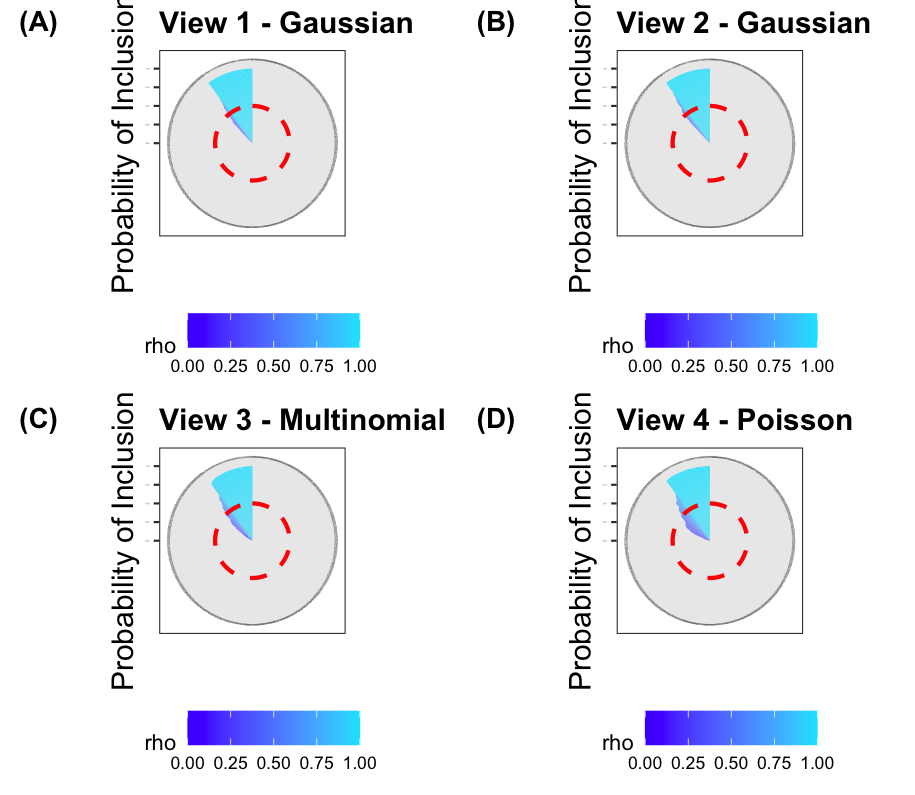
\includegraphics[width=0.7\textwidth]{../results/piplot_sim_data.png}
  \caption{PIP plot showing the posterior inclusion probabilities (PIPs) of features across all data views.}
  \label{fig:piplot}
\end{figure}

Figure~\ref{fig:piplot} illustrates the posterior probability of variable inclusion across
 the four different data views: (A) and (B) correspond to the two Gaussian views, 
 (C) corresponds to the Multinomial view, and (D) to the Poisson view.
  In each subplot, the radial axis represents the probability of inclusion for individual variables,
   with higher values indicating stronger evidence of variable relevance.
    The angular separation reflects the clustering structure among variables.

The color gradient encodes the \(\rho\) value, which governs the correlation or dependence strength across features. Bright blue regions (high \(\rho\)) indicate confidently selected variables, while darker tones indicate low inclusion probability or noise. Across all views, the most informative variables are highlighted clearly with high inclusion probabilities concentrated in narrow angular bands, consistent with the true signal structure of the simulated dataset.


\begin{figure}[!h]
  \centering
  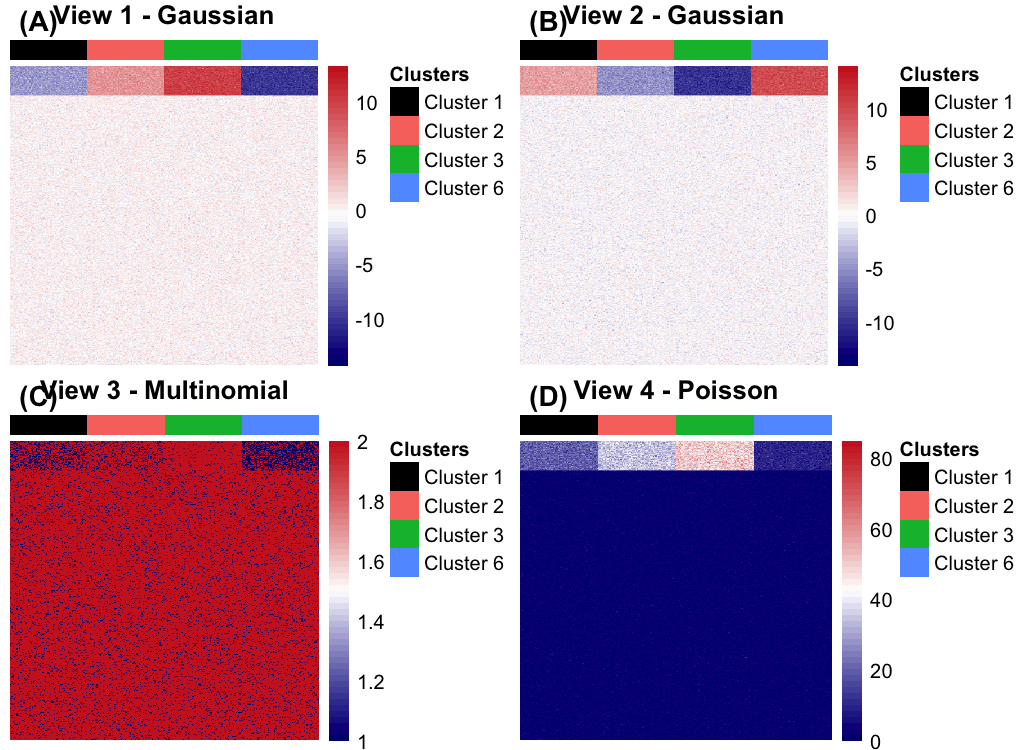
\includegraphics[width=0.7\textwidth]{../results/hamp_sim_data.png}
  \caption{Cluster heatmap showing the clustering structure and variable selection across all data views.}
  \label{fig:chmap_sim_data}
\end{figure}

Figure~\ref{fig:chmap_sim_data} shows heatmaps of the four data views used for clustering. 
Clear block patterns in Views 1 and 2 (Gaussian) indicate that these features distinguish clusters well. 
View 3 (Multinomial) also displays cluster-specific structure in the upper rows. 
While View 4 (Poisson) is mostly sparse, the top block shows variation across clusters, suggesting some informative features. 
Together, these heatmaps validate that each view contributes to identifying distinct clusters.

% ----------------above are moved to vscode for refining--------
\section{iClusterVB Implementation on Breast Cancer data}

In this section, we transition from working with simulation data to applying our
methodology to a more realistic dataset. 

Specifically, we utilize the Breast Cancer dataset obtained from Kaggle.
This dataset provides a practical context to evaluate the performance 
and applicability of the iClusterVB implementation in addressing real-world challenges.


There are no missing values in the dataset, and all features are numeric(except the target variable(M \& B)), which provide 
us convenient conditions for applying the iClusterVB method.

Before taking statistical testing, we did some data preprocessing. We encoded the target variable and split the data based on the 
target variable, got two subsets of data, one for M and one for B.  After checking the distributions of the two data sets,
we found there were heavy skewness and outliers in the data, therefore we make a simple logarithm transformation on the data
\footnote{In later practice, other transfomration can be used here, taking log-transfomration is only for convenience of demonstration
here}.

\subsection{Distribution Testing}
By normality testing, we found that most variables are not normally distributed,
only four variables are normally distributed, which are: \textit{area\_se, texture\_worst, concave points\_worst, symmetry\_worst}.

\begin{figure}[!h]
    \centering
    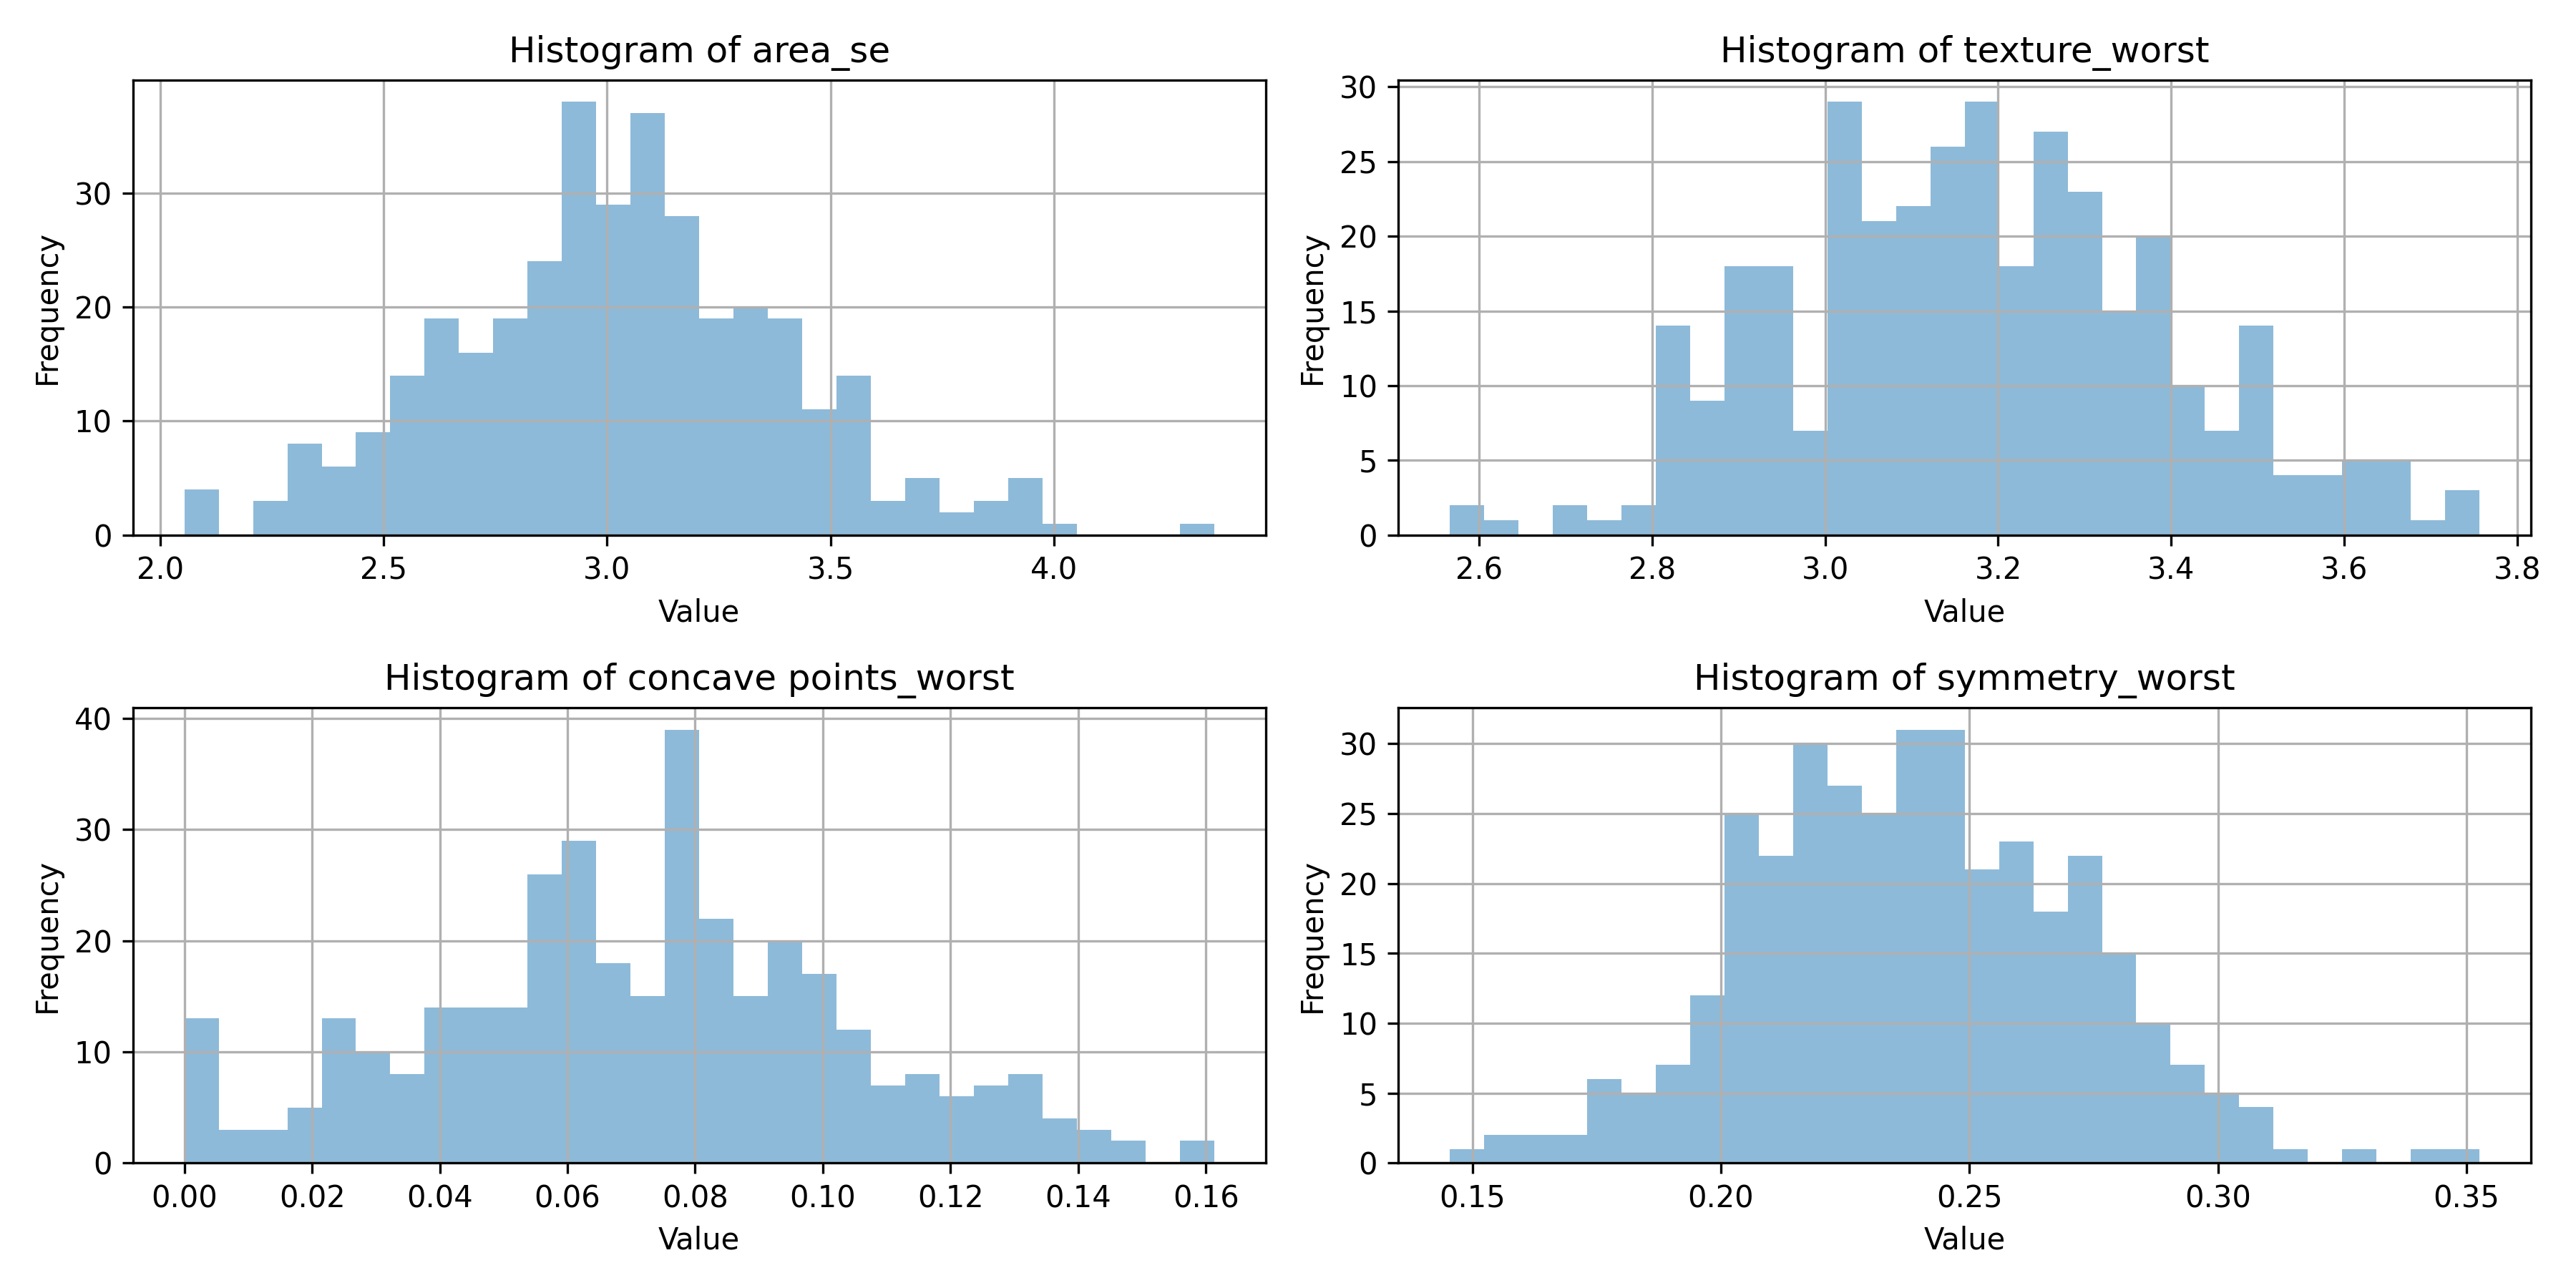
\includegraphics[width=0.9\linewidth]{../results/breast_cancer_normal_distributions.png}
    \caption{Histograms of normal distributions that pass the normality test(corresponding to table \ref{tab:normality_brca})}
    \label{fig:normal_histograms_brca}
\end{figure}

Hence, we will take these four variables as valid normally distributed features as one of the inputs for the iClusterVB method.


We also did Poisson testing on the data, and we found that most variables are not Poisson distributed, 
only one variable \textit{texture\_se} is Poisson distributed.

\begin{table}[!h]
    \centering
    \caption{Chi-square test for all variables in the breast cancer dataset}
    \label{tab:chi_square_brca}
    \begin{tabular}{cccc}
    \toprule
    \textbf{index} & \textbf{Variable} & \textbf{Chi2 Statistic} & \textbf{Poisson-p-value} \\
    \midrule
    3 & texture\_mean & 25.2086 & 0.0000 \\
    4 & perimeter\_mean & 334.8591 & 0.0000 \\
    5 & area\_mean & 232.2412 & 0.0000 \\
    13 & texture\_se & 1.5309 & 0.2160 \\
    14 & perimeter\_se & 63.7165 & 0.0000 \\
    15 & area\_se & 108.8869 & 0.0000 \\
    22 & radius\_worst & 235.0098 & 0.0000 \\
    23 & texture\_worst & 137.9469 & 0.0000 \\
    24 & perimeter\_worst & 353.2600 & 0.0000 \\
    25 & area\_worst & 354.8223 & 0.0000 \\
    \bottomrule
    \end{tabular}
\end{table}

Other variables that are not shown in the table are not suitable for the Poission test, and we assumed they are not Poisson distributed.

To multinomial(bernoulli) test, we found that all variables are not interget-valued, hence they are not suitable for multinomial test.
Therefore, we will not take multinomial test in this case.


\begin{table}[!h]
    \centering
    \caption{Variables Selected for iClusterVB Analysis}
    \label{tab:variables_iclustervb}
    \begin{tabular}{ll}
    \toprule
    \textbf{Variable Type} & \textbf{Selected Variables} \\
    \midrule
    Gaussian (Normal) & area\_se, texture\_worst, concave points\_worst, symmetry\_worst \\
    Poisson & texture\_se \\
    \bottomrule
    \end{tabular}
\end{table}

Table~\ref{tab:variables_iclustervb} lists the variables selected for the iClusterVB analysis. 
The Gaussian variables were chosen based on their normality test results, while the Poisson variable was selected 
based on the Poisson test. These variables serve as inputs for the iClusterVB method, representing distinct data views 
to capture meaningful patterns and relationships in the dataset.


\subsection{iClusterVB Results}

\subsection*{Clustering Summary on Breast Cancer Subset}

The clustering algorithm was applied to a real subset of the breast cancer dataset, yielding the following results:

\begin{table}[!h]
    \centering
    \caption{Clustering Summary for Breast Cancer Subset}
    \label{tab:brca_clustering_summary}
    \begin{tabular}{ll}
    \toprule
    \textbf{Metric} & \textbf{Result} \\
    \midrule
    Total number of individuals & 357 \\
    Maximum number of clusters (user input) & 6 \\
    Number of clusters determined & 6 \\
    \midrule
    Variables selected (posterior inclusion probability > 0.5) & \\
    \quad View 1 - Gaussian & 2 out of 4 \\
    \quad View 2 - Poisson & 2 out of 2 \\
    \bottomrule
\end{tabular}
    
    \vspace{1em}

\begin{tabular}{cccccc}
    \multicolumn{6}{c}{\textbf{Cluster Membership Distribution}} \\
    \toprule
    Cluster 1 & Cluster 2 & Cluster 3 & Cluster 4 & Cluster 5 & Cluster 6 \\
    \midrule
    57 & 55 & 80 & 46 & 98 & 21 \\
    \bottomrule
    \end{tabular}
\end{table}

Table~\ref{tab:brca_clustering_summary} presents the clustering summary for a subset of the breast cancer dataset. 
The algorithm successfully identified 6 clusters from 357 individuals, matching the user-specified maximum number of clusters. 
Cluster sizes ranged from 21 to 98. Variable selection results show that 2 out of 4 Gaussian variables and all 2 Poisson variables were selected based on a posterior inclusion probability threshold of 0.5, 
indicating their importance in distinguishing clusters across the two views.

Figure~\ref{fig:breast_cancer_heatmap} shows the clustering heatmaps for the breast cancer dataset based on two data views: 
(A) Gaussian and (B) Poisson. Each column corresponds to an individual, and rows represent variables.
 The color bars at the top denote the cluster membership of each individual. In both views, clear block patterns are observed,
  indicating distinct variable activity across different clusters. This separation suggests that the clustering algorithm effectively 
  identified subgroups with different underlying characteristics in both Gaussian and Poisson features.

\begin{figure}
    \centering
    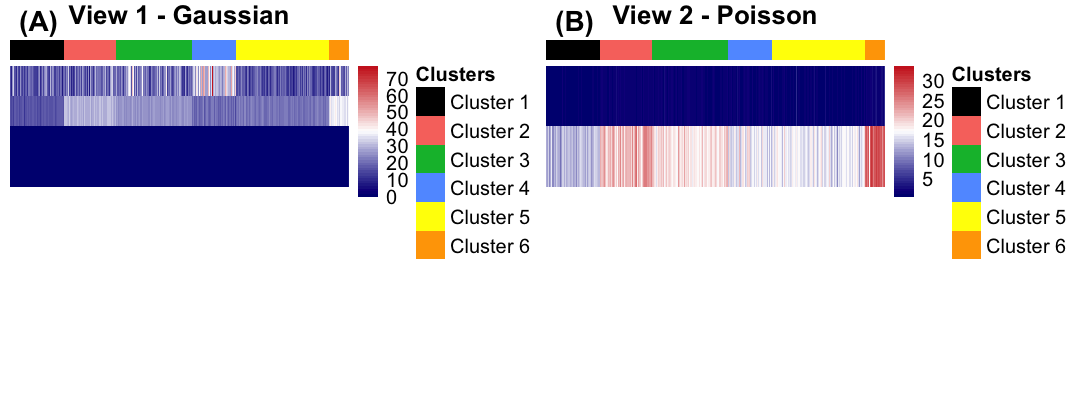
\includegraphics[width=0.9\linewidth]{../results/hamp_real_data.png}
    \caption{Heatmap of the clustering results on breast cancer data}
    \label{fig:breast_cancer_heatmap}
\end{figure}
% \section{Results}
We applied iClusterVB on simulated data with 100 individuals across four data views. The model accurately determined $K=3$, consistent with ground truth. Cluster sizes were:
\begin{itemize}
  \item Cluster 1: 20 individuals
  \item Cluster 2: 23 individuals
  \item Cluster 3: 57 individuals
\end{itemize}

This demonstrated high accuracy in subgroup detection. Feature selection was not activated but could be useful in further analyses.

% \section{Conclusion}
\begin{itemize}
  \item \textbf{Summary of Findings:} iClusterVB effectively clusters high-dimensional, mixed-type data, demonstrating robust performance across various datasets. It provides meaningful insights into the underlying structure of complex data, enabling the identification of distinct subgroups.
  \item \textbf{Practical Implications:} The method is particularly useful for multi-omics studies, biomarker discovery, and patient stratification, offering a scalable and interpretable approach for integrating diverse data types. This can aid in personalized medicine and targeted therapeutic strategies.
  \item \textbf{Future Directions:} Future work could explore supervised modeling with subtype labels to enhance predictive accuracy. Additionally, applying iClusterVB to other real-world cancer datasets or extending it to incorporate temporal or spatial data could further validate its utility and expand its applications.
\end{itemize}

\clearpage
\section{Appendix}

% \subsection{R code-1}
% \begin{lstlisting}[language=R, caption=R code example]
% # Load the iClusterVB package
% library(iClusterVB)
% # Load the cowplot library to combine plots
% library(cowplot)

% # Part 1: simulation data
% # Load the built-in simulated data
% get(data("sim_data"))

% # Create a list of data views from the simulated dataset
% list_sim_data <- list(
%   gauss_1 = sim_data$continuous1_data,
%   gauss_2 = sim_data$continuous2_data,
%   multinomial_1 = sim_data$binary_data,
%   poisson_1 = sim_data$count_data
% )

% # Re-code 0's to 2's for the multinomial data (iClusterVB requires non-zero values)
% list_sim_data$multinomial_1[list_sim_data$multinomial_1 == 0] <- 2

% # Optional: check first few rows of each dataset
% head(list_sim_data$gauss_1[, 1:6])
% head(list_sim_data$gauss_2[, 1:6])
% head(list_sim_data$multinomial_1[, 1:6])
% head(list_sim_data$poisson_1[, 1:6])

% # Specify the distribution for each view
% dist_sim_data <- c("gaussian", "gaussian", "multinomial", "poisson")

% # Run the iClusterVB model on the simulated data
% set.seed(123)
% fit_sim_data <- iClusterVB(
%   mydata = list_sim_data,
%   dist = dist_sim_data,
%   K = 8,  # max clusters to allow algorithm to reduce
%   initial_method = "VarSelLCM",
%   VS_method = 1,  # enable feature selection
%   max_iter = 100
% )

% # Summarize the fitted model
% summary(fit_sim_data, rho = 0.5)

% # Compare estimated clusters with ground truth
% table(fit_sim_data$cluster, sim_data$cluster_true)

% # plot piplot
% piplot(fit_sim_data , nrow = 2, ncol = 2, align = "hv ")

% # Generate cluster-specific heatmaps from iClusterVB results
% hmaps_sim <- chmap(
%   fit_sim_data,
%   rho = 0,
%   cols = c(
%     "#000000",  # black
%     "#F8766D",  # reddish-pink
%     "#00BA38",  # green
%     "#619CFF"   # blue
%   ),
%   scale = "none"  # no scaling applied to preserve original feature scale
% )

% # Arrange the generated heatmaps in a 2x2 grid layout
% plot_grid(
%   plotlist = hmaps_sim,
%   ncol = 2,
%   nrow = 2,
%   labels = c("(A)", "(B)", "(C)", "(D)")
% )

% \end{lstlisting}

% \subsection{R code-BRCA TCG}
% \begin{lstlisting}[language=R, caption=R code example]
% ```{r}
% # Load and transpose breast cancer data from CSV files 
% gene_exp <- read.csv(file = "C:...Project2/Breast-TCGA/Breast-TCGA/context1_GE.csv", header = TRUE, row.names = 1)
% gene_exp <- t(gene_exp)

% methy_exp <- read.csv(file = "C:...Project2/Breast-TCGA/Breast-TCGA/context2_Meth.csv", header = TRUE, row.names = 1)
% methy_exp <- t(methy_exp)

% mirna_exp <- read.csv(file = "C:...Project2/Breast-TCGA/Breast-TCGA/context3_miRNA.csv", header = TRUE, row.names = 1)
% mirna_exp <- t(mirna_exp)

% # Load clinical/survival data
% clinical <- read.csv(file = "C:/Users/hadis/OneDrive/Documents/seminar/Project2/Breast-TCGA/Breast-TCGA/Table1Nature.csv", header = TRUE)


% # Extract  PatientID 
% id <- sub("TCGA-\\w+-(\\w+)", "\\1", clinical$PatientID)
% clinical$id <- id

% # Scale the data
% gene_exp_scale <- apply(gene_exp, 2, scale)
% methy_exp_scale <- apply(methy_exp, 2, scale)
% mirna_exp_scale <- apply(mirna_exp, 2, scale)

% # Combine into a list for iClusterVB input
% list_brca_data <- list(
%   gene_exp_scale,
%   methy_exp_scale,
%   mirna_exp_scale
% )

% # Specify data distribution for each view
% dist_brca_data <- c("gaussian", "gaussian", "gaussian")

% library("iClusterVB")

% set.seed(20204)  

% fit_brca <- iClusterVB(
%   mydata = list_brca_data,
%   dist = dist_brca_data,
%   K = 6,                        
%   initial_method = "VarSelLCM",
%   initial_vs_prob = 0.1,       # Prior probability of variable selection
%   max_iter = 100,              # Max iterations for convergence
%   VS_method = 1,               
%   per = 100                   
% )

% summary(fit_brca)

% library(ggplot2)

% var_gene <- apply(gene_exp_scale, 2, var)
% var_methy <- apply(methy_exp_scale, 2, var)
% var_mirna <- apply(mirna_exp_scale, 2, var)

% df_var <- data.frame(
%   variance = c(var_gene, var_methy, var_mirna),
%   type = c(rep("Gene", length(var_gene)), rep("Methy", length(var_methy)), rep("miRNA", length(var_mirna)))
% )

% ggplot(df_var, aes(x = variance, fill = type)) +
%   geom_histogram(bins = 50, alpha = 0.7, position = "identity") +
%   scale_x_log10() +
%   theme_minimal() +
%   ggtitle("Feature Variance Distribution Across Omics")

% library(pheatmap)

% pheatmap(cor(t(gene_exp_scale)), show_rownames = FALSE, show_colnames = FALSE, main = "Sample Correlation - Gene Exp")
% pheatmap(cor(t(methy_exp_scale)), show_rownames = FALSE, show_colnames = FALSE, main = "Sample Correlation - Methylation")
% pheatmap(cor(t(mirna_exp_scale)), show_rownames = FALSE, show_colnames = FALSE, main = "Sample Correlation - miRNA")


% pca_plot <- function(data, title) {
%   pca <- prcomp(data, center = TRUE, scale. = TRUE)
%   pca_df <- data.frame(PC1 = pca$x[,1], PC2 = pca$x[,2])
  
%   ggplot(pca_df, aes(x = PC1, y = PC2)) +
%     geom_point(alpha = 0.6) +
%     ggtitle(title) +
%     theme_minimal()
% }

% pca_plot(gene_exp_scale, "PCA - Gene Expression")
% pca_plot(methy_exp_scale, "PCA - Methylation")
% pca_plot(mirna_exp_scale, "PCA - miRNA Expression")

% \end{lstlisting}


\subsection{Tables}

\begin{table}[!h]
\centering
\caption{Normality test for Gaussian distribution (first 1000 columns in the simulation data)}
\label{tab:normal_metrics}
\begin{tabular}{r l r r r}
\toprule
\textbf{Index} & \textbf{Variable} & \textbf{Skewness} & \textbf{Kurtosis} & \textbf{Normality p-value} \\
\midrule
0  & gauss\_2\_396 & -0.1079 & -0.0766 & 0.7817 \\
1  & gauss\_1\_225 & 0.0277 & -0.1564 & 0.9313 \\
2  & gauss\_2\_18  & -0.0052 & -1.5656 & 0.0000 \\
3  & gauss\_1\_90  & -0.1858 & 0.3446  & 0.2363 \\
4  & gauss\_1\_375 & 0.0521  & -0.0305 & 0.9374 \\
5  & gauss\_2\_217 & -0.0205 & -0.1222 & 0.9708 \\
6  & gauss\_1\_490 & 0.0701  & -0.0306 & 0.8950 \\
7  & gauss\_1\_260 & -0.0380 & 0.0563  & 0.8946 \\
8  & gauss\_1\_124 & 0.1376  & -0.2938 & 0.4495 \\
9  & gauss\_1\_400 & -0.1274 & -0.3238 & 0.4176 \\
10 & gauss\_1\_167 & 0.1571  & -0.3698 & 0.2736 \\
11 & gauss\_1\_18  & -0.0073 & -1.5921 & 0.0000 \\
12 & gauss\_1\_318 & 0.0031  & 0.1366  & 0.8125 \\
13 & gauss\_1\_220 & 0.1701  & -0.4797 & 0.1043 \\
14 & gauss\_1\_308 & -0.0471 & -0.3887 & 0.3883 \\
15 & gauss\_1\_385 & 0.0960  & -0.1883 & 0.7422 \\
16 & gauss\_2\_210 & 0.0282  & 0.3164  & 0.5181 \\
17 & gauss\_2\_354 & -0.0808 & 0.2698  & 0.5219 \\
18 & gauss\_1\_369 & 0.0930  & 0.0298  & 0.7920 \\
19 & gauss\_1\_147 & -0.2302 & 0.1885  & 0.2441 \\
20 & gauss\_1\_50  & -0.0317 & -1.6111 & 0.0000 \\
21 & gauss\_1\_405 & -0.0403 & 0.0832  & 0.8590 \\
22 & gauss\_1\_117 & 0.0661  & -0.3219 & 0.5403 \\
23 & gauss\_2\_179 & -0.0018 & -0.3278 & 0.5762 \\
24 & gauss\_2\_249 & 0.3049  & 0.6479  & 0.0258 \\
25 & gauss\_1\_68  & -0.1215 & -0.1024 & 0.7268 \\
26 & gauss\_1\_299 & 0.2415  & -0.1434 & 0.2882 \\
27 & gauss\_1\_118 & -0.2193 & 0.0210  & 0.3537 \\
28 & gauss\_2\_48  & 0.0079  & -1.5732 & 0.0000 \\
29 & gauss\_2\_484 & 0.1617  & -0.2456 & 0.4565 \\
\bottomrule
\end{tabular}
\end{table}


\begin{table}[!h]
\centering
\caption{Poisson test for Poisson distribution (1500 to 2000 columns in the simulation data)}
\label{tab:poisson_metrics}
\begin{tabular}{r l r r}
\toprule
\textbf{Index} & \textbf{Variable} & \textbf{Statistic} & \textbf{Poisson p-value} \\
\midrule
0  & poisson\_1\_347 & 8.1418 & 0.4197 \\
1  & poisson\_1\_130 & 3.3996 & 0.8457 \\
2  & poisson\_1\_278 & 2.0546 & 0.9568 \\
3  & poisson\_1\_31  & 1896309619.6291 & 0.0000 \\
4  & poisson\_1\_233 & 2.1521 & 0.9509 \\
5  & poisson\_1\_405 & 7.6532 & 0.3642 \\
6  & poisson\_1\_343 & 4.8117 & 0.6829 \\
7  & poisson\_1\_458 & 4.6286 & 0.5923 \\
8  & poisson\_1\_336 & 9.0090 & 0.3415 \\
9  & poisson\_1\_222 & 7.1677 & 0.4116 \\
10 & poisson\_1\_440 & 6.7327 & 0.3463 \\
11 & poisson\_1\_357 & 7.3086 & 0.3975 \\
12 & poisson\_1\_341 & 9.9632 & 0.1907 \\
13 & poisson\_1\_113 & 5.7099 & 0.4565 \\
14 & poisson\_1\_420 & 1.8409 & 0.9337 \\
15 & poisson\_1\_447 & 12.7249 & 0.0476 \\
16 & poisson\_1\_248 & 7.0096 & 0.5356 \\
17 & poisson\_1\_417 & 7.0637 & 0.2159 \\
18 & poisson\_1\_194 & 2.7987 & 0.8337 \\
19 & poisson\_1\_9   & 6684971.6159 & 0.0000 \\
20 & poisson\_1\_61  & 2.9649 & 0.8132 \\
21 & poisson\_1\_22  & 952499618.9309 & 0.0000 \\
22 & poisson\_1\_407 & 0.9116 & 0.9887 \\
23 & poisson\_1\_282 & 41.5326 & 0.0000 \\
24 & poisson\_1\_129 & 8.1200 & 0.4218 \\
25 & poisson\_1\_421 & 7.0042 & 0.4284 \\
26 & poisson\_1\_204 & 24.9668 & 0.0008 \\
27 & poisson\_1\_427 & 3.0758 & 0.8779 \\
28 & poisson\_1\_258 & 10.4206 & 0.1080 \\
29 & poisson\_1\_383 & 5.0726 & 0.6511 \\
\bottomrule
\end{tabular}
\end{table}

\begin{table}[!h]
\centering
\caption{Bernoulli test for Bernoulli distribution (1000 to 1500 columns in the simulation data)}
\label{tab:bernoulli_metrics}
\begin{tabular}{ccccccc}
\toprule
\textbf{Index} & \textbf{Variable} & \textbf{Chi2 Statistic} & \textbf{p-value} & \textbf{Estimated $p$} & \textbf{\# 0s} & \textbf{\# 1s} \\
\midrule
0 & multinomial\_1\_353 & 0.7407 & 0.3894 & 0.1167 & 212 & 28 \\
1 & multinomial\_1\_345 & 1.6667 & 0.1967 & 0.0750 & 222 & 18 \\
2 & multinomial\_1\_196 & 1.6667 & 0.1967 & 0.0750 & 222 & 18 \\
3 & multinomial\_1\_103 & 1.1574 & 0.2820 & 0.1208 & 211 & 29 \\
4 & multinomial\_1\_83 & 1.1574 & 0.2820 & 0.0792 & 221 & 19 \\
5 & multinomial\_1\_499 & 1.6667 & 0.1967 & 0.0750 & 222 & 18 \\
6 & multinomial\_1\_22 & 106.6667 & 0.0000 & 0.3000 & 168 & 72 \\
7 & multinomial\_1\_138 & 0.4167 & 0.5186 & 0.0875 & 219 & 21 \\
8 & multinomial\_1\_360 & 4.6296 & 0.0314 & 0.1417 & 206 & 34 \\
9 & multinomial\_1\_72 & 0.7407 & 0.3894 & 0.1167 & 212 & 28 \\
10 & multinomial\_1\_486 & 0.0000 & 1.0000 & 0.1000 & 216 & 24 \\
11 & multinomial\_1\_101 & 2.9630 & 0.0852 & 0.0667 & 224 & 16 \\
12 & multinomial\_1\_90 & 0.0463 & 0.8296 & 0.0958 & 217 & 23 \\
13 & multinomial\_1\_42 & 161.1574 & 0.0000 & 0.3458 & 157 & 83 \\
14 & multinomial\_1\_271 & 0.0463 & 0.8296 & 0.0958 & 217 & 23 \\
15 & multinomial\_1\_252 & 0.0000 & 1.0000 & 0.1000 & 216 & 24 \\
16 & multinomial\_1\_110 & 0.7407 & 0.3894 & 0.1167 & 212 & 28 \\
17 & multinomial\_1\_415 & 0.7407 & 0.3894 & 0.1167 & 212 & 28 \\
18 & multinomial\_1\_122 & 0.7407 & 0.3894 & 0.0833 & 220 & 20 \\
19 & multinomial\_1\_230 & 0.4167 & 0.5186 & 0.0875 & 219 & 21 \\
20 & multinomial\_1\_403 & 1.6667 & 0.1967 & 0.0750 & 222 & 18 \\
21 & multinomial\_1\_88 & 0.4167 & 0.5186 & 0.1125 & 213 & 27 \\
22 & multinomial\_1\_126 & 7.8241 & 0.0052 & 0.1542 & 203 & 37 \\
23 & multinomial\_1\_130 & 1.1574 & 0.2820 & 0.0792 & 221 & 19 \\
24 & multinomial\_1\_439 & 0.4167 & 0.5186 & 0.1125 & 213 & 27 \\
25 & multinomial\_1\_16 & 89.6296 & 0.0000 & 0.2833 & 172 & 68 \\
26 & multinomial\_1\_340 & 3.7500 & 0.0528 & 0.1375 & 207 & 33 \\
27 & multinomial\_1\_293 & 0.0000 & 1.0000 & 0.1000 & 216 & 24 \\
28 & multinomial\_1\_64 & 0.0000 & 1.0000 & 0.1000 & 216 & 24 \\
29 & multinomial\_1\_82 & 0.4167 & 0.5186 & 0.0875 & 219 & 21 \\
\bottomrule
\end{tabular}
\end{table}

\begin{table}[!h]
    \centering
    \caption{Normality test for all variables in the breast cancer dataset}
    \label{tab:normality_brca}
    \begin{tabular}{r l r r r}
        \toprule
        \textbf{Index} & \textbf{Variable} & \textbf{Skewness} & \textbf{Kurtosis} & \textbf{Normality $p$-value} \\
        \midrule
        0  & id                        & 6.9517 & 48.7647 & 0.0000 \\
        1  & radius\_mean              & -0.4930 & 0.2500 & 0.0006 \\
        2  & texture\_mean             & 0.3480 & 0.1690 & 0.0207 \\
        3  & perimeter\_mean           & -0.5277 & 0.3695 & 0.0002 \\
        4  & area\_mean                & -0.5650 & 0.3883 & 0.0001 \\
        5  & smoothness\_mean          & 0.6002 & 1.5932 & 0.0000 \\
        6  & compactness\_mean         & 1.0849 & 1.7566 & 0.0000 \\
        7  & concavity\_mean           & 2.9089 & 15.0911 & 0.0000 \\
        8  & concave points\_mean      & 0.8717 & 0.8859 & 0.0000 \\
        9  & symmetry\_mean            & 0.5683 & 1.0837 & 0.0000 \\
        10 & fractal\_dimension\_mean  & 1.6090 & 4.2304 & 0.0000 \\
        11 & radius\_se                & 1.1020 & 2.0694 & 0.0000 \\
        12 & texture\_se               & 0.5976 & 0.5768 & 0.0000 \\
        13 & perimeter\_se             & 0.5015 & -0.0299 & 0.0009 \\
        14 & area\_se                  & 0.1348 & 0.2530 & 0.3185 \\
        15 & smoothness\_se            & 1.4897 & 2.9455 & 0.0000 \\
        16 & compactness\_se           & 2.1325 & 5.4932 & 0.0000 \\
        17 & concavity\_se             & 5.4665 & 45.6831 & 0.0000 \\
        18 & concave points\_se        & 2.0728 & 9.9365 & 0.0000 \\
        19 & symmetry\_se              & 1.3380 & 3.0752 & 0.0000 \\
        20 & fractal\_dimension\_se    & 4.2709 & 26.7974 & 0.0000 \\
        21 & radius\_worst             & -0.4131 & 0.0001 & 0.0073 \\
        22 & texture\_worst            & 0.1375 & -0.2272 & 0.3988 \\
        23 & perimeter\_worst          & -0.4131 & 0.0143 & 0.0072 \\
        24 & area\_worst               & -0.4709 & 0.0885 & 0.0017 \\
        25 & smoothness\_worst         & 0.2805 & 0.2833 & 0.0477 \\
        26 & compactness\_worst        & 0.8333 & 0.8487 & 0.0000 \\
        27 & concavity\_worst          & 1.6051 & 5.2030 & 0.0000 \\
        28 & concave points\_worst     & 0.0221 & -0.2058 & 0.7610 \\
        29 & symmetry\_worst           & 0.1265 & 0.1762 & 0.4333 \\
        30 & fractal\_dimension\_worst & 1.3515 & 2.8535 & 0.0000 \\
        \bottomrule
    \end{tabular}
\end{table}







\end{document}